\section{Introduction}

Motion planning is a fundamental problem in robotics that involves computing a feasible and efficient trajectory for a robot to move from an initial configuration to a goal configuration while satisfying various constraints\cite{lavalle2006planning}.
%
The problem becomes particularly challenging in high dimensional systems, which are generally known to be PSPACE-hard\cite{reif1979complexity}.

Classical approaches to motion planning rely heavily on sampling-based planners, such as Rapidly-exploring Random Trees (RRT)\cite{lavalle2001randomized} and Probabilistic Roadmaps (PRM)\cite{kavraki1996probabilistic}, due to their ability to efficiently explore high-dimensional spaces.
%
These planners have been widely adopted because they can handle complex environments without requiring an explicit representation of the free space.
%
However, when additional constraints such as kinodynamic feasibility, obstacle avoidance, or motion continuity are introduced, these methods struggle to produce high-quality, optimal trajectories.

Recent advances in optimization-based motion planning have tackled these limitations by formulating the problem as a compact mixed-integer convex program\cite{marcucci2023motion}.
%
One such approach, the Graph of Convex Sets (GCS) framework\cite{marcucci2024shortest}, enables the encoding of collision-avoidance constraints and system dynamics within a single convex optimization formulation.
%
By leveraging convex relaxations and mixed-integer programming, GCS provides a structured way to computing globally optimal trajectories while ensuring feasibility in constrained environments.

\begin{figure}[!t]
    \centering
    \begin{subfigure}[b]{0.19\textwidth}
        \centering
        \fbox{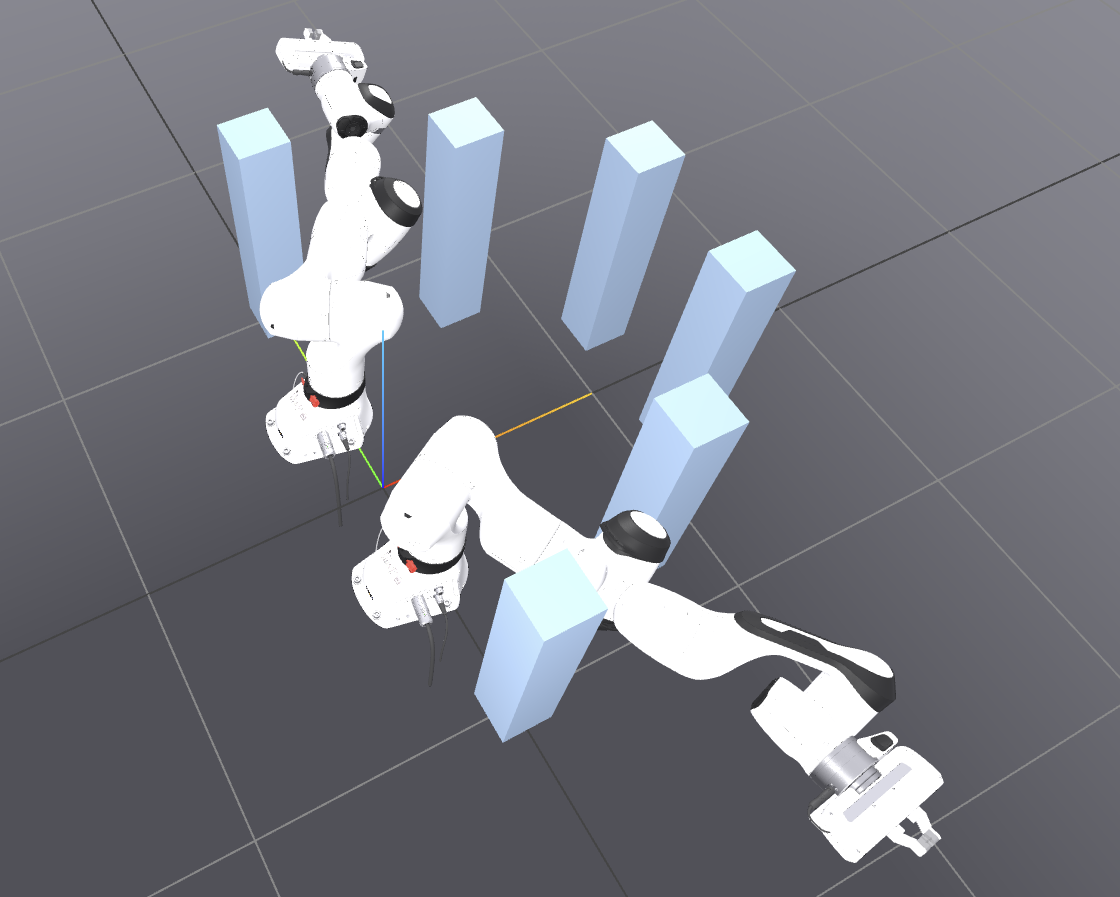
\includegraphics[width=\textwidth]{figures/cage_start_orbit.png}}
        \captionsetup{justification=centering}
        \caption{Start configuration}
        \label{subfig:cage_start_orbit}
    \end{subfigure}\hspace{0.01\textwidth}
    \begin{subfigure}[b]{0.19\textwidth}
        \centering
        \fbox{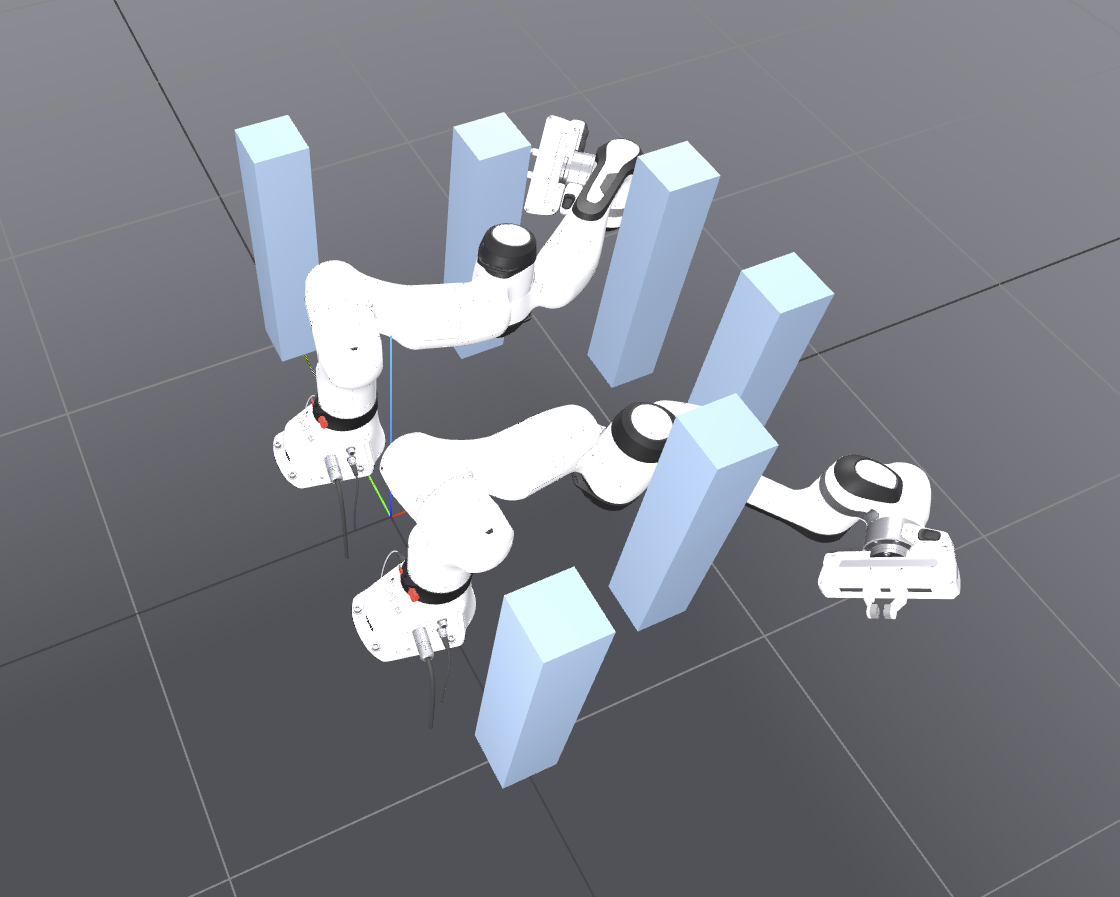
\includegraphics[width=\textwidth]{figures/cage_goal_orbit.png}}
        \captionsetup{justification=centering}
        \caption{Goal configuration}
        \label{subfig:cage_goal_orbit}
    \end{subfigure}
    \caption{A dual-arm manipulation problem for two Franka Emika Panda robots in $\mathbb{R}^{14}$, simulated in Drake. The robots start in an initial configuration (a) positioned between the first two rows of obstacles and must reach the goal configuration (b) between the last two rows of obstacles without collisions.}
    \label{fig:simulation}
\end{figure}

\subsection{Contributions}
In this project, we explore the use of the GCS framework for kinodynamic motion planning in dual-arm robotic manipulation.
%
Our key contributions include:
\begin{itemize}
    \item We formulate the problem of finding \textit{collision-free, kinodynamic motion plans} for a dual-arm manipulator as a mixed-integer convex program, similar to~\cite{marcucci2023motion}.
    %
    Unlike prior work, our study considers the scalability of the framework in significantly higher-dimensional systems---14 degrees of freedom in this case (Figure~\ref{fig:simulation}).
    %
    \item We extensively evaluate our optimization-based approach against classical sampling-based motion planners from the Open Motion Planning Library (OMPL)~\cite{sucan2012open}, analyzing key performance metrics such as computation time, solution quality, and success rate.
\end{itemize}

This report is organized as follows: